\documentclass[10pt,a4paper]{extarticle}
\usepackage[latin1]{inputenc}
\usepackage{amsmath}
\usepackage{microtype}
\usepackage[none]{hyphenat}
\usepackage{verbatim}
\usepackage{amsfonts}
\usepackage{amssymb}
\usepackage{enumitem}
\renewcommand{\familydefault}{\sfdefault}
\usepackage{mathpazo}
\renewcommand{\rmdefault}{put}
\usepackage{enumitem}
\usepackage[dvipsnames,svgnames]{xcolor}
\usepackage{tkz-euclide}
\usetkzobj{all}
\usepackage{graphicx}
\usepackage{tikz} 	
\usepackage{adjustbox}
\usepackage{multicol}
\usepackage{lipsum}
\usepackage[left=0.7cm,right=1cm,top=1cm,bottom=1.5cm]{geometry}
\usepackage{cancel} \usepackage{xcolor}
\usepackage{tcolorbox}
\usetikzlibrary{decorations.pathmorphing,patterns}
\usetikzlibrary{decorations.pathreplacing,calc}
 \newcommand\coret[2][red]{\renewcommand\CancelColor{\color{#1}}\cancel{#2}}
\SetLabelAlign{Center}{\hfil\makebox[1.0em]{#1}\hfil}

%%_------= solusi


% Set this =0 to hide, =1 to show

% Set this =0 to hide, =1 to show
\newtcolorbox{mybox}[1][] { colframe = blue!10, colback = blue!3,boxsep=0pt,left=0.2em, coltitle = blue!20!black, title = \textbf{jawab}, #1, } 

%---------- kunci (jika 1 ) muncul
\def\tampilkunci{1}
\newcommand{\hide}[1]{\ifnum\tampilkunci=1
%
\begin{mybox}
 #1
\end{mybox}
%
\vspace{\baselineskip}\fi}



\newcommand*\cicled[1]{\tikz[baseline=(char.base)]{\node[white, shape=circle, fill=red!80,draw,inner sep=0.5pt](char){#1};}}

\newcommand*\kunci[1]{\ifnum\tampilkunci=1
%
\tikz[baseline=(char.base)]{\node[red, shape=circle,draw,inner sep=0.5pt,xshift=2pt](char){#1};}\stepcounter{enumii}
\fi\ifnum\tampilkunci=0
%
\hspace{3pt}#1\stepcounter{enumii}
%
\fi}

\newcommand*\silang[1]{\tikz[baseline=(char.base)]{
\draw[red,thick](-0.2,-0.20)--(0.2,0.2);
\draw[red,thick](-0.2,0.20)--(0.2,-0.2);
\node[black](char){#1};
}}

\newcommand*\centang[1]{\tikz[baseline=(char.base)]{
\draw[red, very thick](-0.2,0.1)--(-0.1,0)--(0.2,0.3);
\node(char){#1};
}}

\newcommand*\merah[1]{
\textcolor{red}{#1}}
\newcommand*\pilgan[1]{
\begin{enumerate}[label=\Alph*., itemsep=0pt,topsep=0pt,leftmargin=*,align=Center] #1 
\end{enumerate}}
\newcommand*\pernyataan[1]{
\begin{enumerate}[label=(\arabic*), itemsep=0pt,topsep=0pt,leftmargin=*] #1 
\end{enumerate}}

\newcommand{\pilgani}[1]{                            \vspace{-0.3cm}\begin{multicols}{2}
 \begin{enumerate}[label=\Alph*., itemsep=0pt,topsep=0pt,leftmargin=*,align=Center]#1                     \end{enumerate}
 \phantom{ini cuma sapi, wedus, dan ayam}
 \end{multicols}}


\begin{document}


 \textbf{Latihan Ulangan Momentum} \phantom{ini nama siswa yang aaamengerjakan soal kuis ini }  

\begin{multicols*}{2}

\begin{enumerate}
\item Dua benda bergerak dengan massa 2 kg dan 4 kg bergerak berlawanan dengan kecepatan 10 m/s dan 15 m/s. Jika setelah tabrakan kecepatan benda 2 kg adalah 2 m/s ke arah berlawanan, maka kecepatan benda 4 kg adalah . . . . . ke arah . . . .
\vspace{3cm}

\item Benda dengan massa 1 kg bergerak searah sumbu $x$ positif dengan kecepatan 10 m/s, benda lain dengan massa sama bergerak ke arah sumbu $y$ positif dengan kecepatan 20 m/s. Maka momentum kedua benda tersebut adalah . .  . .  Ns
\vspace{3.5cm}


\item Benda A bermassa 2 kg bergerak dengan kecepatan 5 m/s membentuk arah 30$^o$ terhadap sumbu $x$ positif. Benda B dengan massa 1 kg bergerak dengan kecepatan $v$ bergerak searah sumbu $y$ negatif. Setelah tabrakan keduanya menempel dan bergerak bersama ke arah sumbu $x$ positif dengan kecepatan 5 m/s. Maka besar $v$ kecepatan benda B adalah . . . . m/s
\vspace{4cm}



\item Dua buah benda massanya 5 kg dan 3 kg bergerak berlawanan arah dengan kecepatan masing-   masing 15 m/s dan 5 m/s .Jika terjadi tumbukan lenting sempurna ,tentukan kecepatan setiap benda setelah tumbukan ?
\vspace{4.5cm}



\item Peluru dengan massa 5 gram ditembakkan pada balok dengan massa 95 gram dalam keadaan diam. Peluru bersarang pada balok dan bergerak bersama dengan kecepatan 5 m/s. Maka kecepatan peluru saat ditembakkan adalah . . .
\vspace{3cm}

\item Peluru dengan massa 5 gram ditembakkan pada balok dengan massa 95 gram dalam keadaan diam. Peluru bersarang pada balok dan bergerak bersama dengan dan naik dengan ketinggian 5 cm. Maka kecepatan peluru saat ditembakkan adalah . . .\\
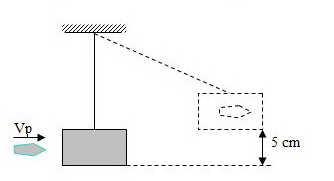
\includegraphics[width=6cm]{pic/latul-mom1} 
\vspace{2cm}



\item Benda 100 gram didorong dengan gaya 300N selama 0,1s. Jika mula-mula diam, kecepatan benda menjadi . . . .
\vspace{2cm}


\item Perhatikan grafik di bawah ini, besarnya impuls yang dilakukan benda selama 3 s adalah . . . \\
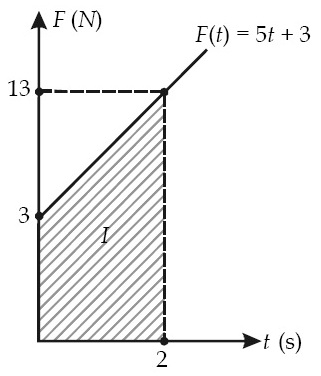
\includegraphics[width=4cm]{pic/latul-mom3} 
\vspace{2cm}

\item Bola dijatuhkan dari ketinggian 100 cm dan memantul setinggi $h$. Jika koefisien restitusi adalah 0,4 maka tinggi $h$ tersebut adalah . . .
\vspace{2cm}

\item Benda A dan B kecepatannya masing-masing 3 dan (-4) m/s. Jika setelah tabrakan menjadi -2m/s dan 1 m/s. Maka koefisien restitusinya adalah . . 
\end{enumerate}
\end{multicols*}\end{document}






